% ============================================================ "exciting cases": switching spin states (Figs 7-9)
\section{Switching spin states}

\begin{frame}{Spin-state crossover by external stimuli (Figure 7)}
  \begin{columns}[c]
    \column{0.42\textwidth}
    \centering
    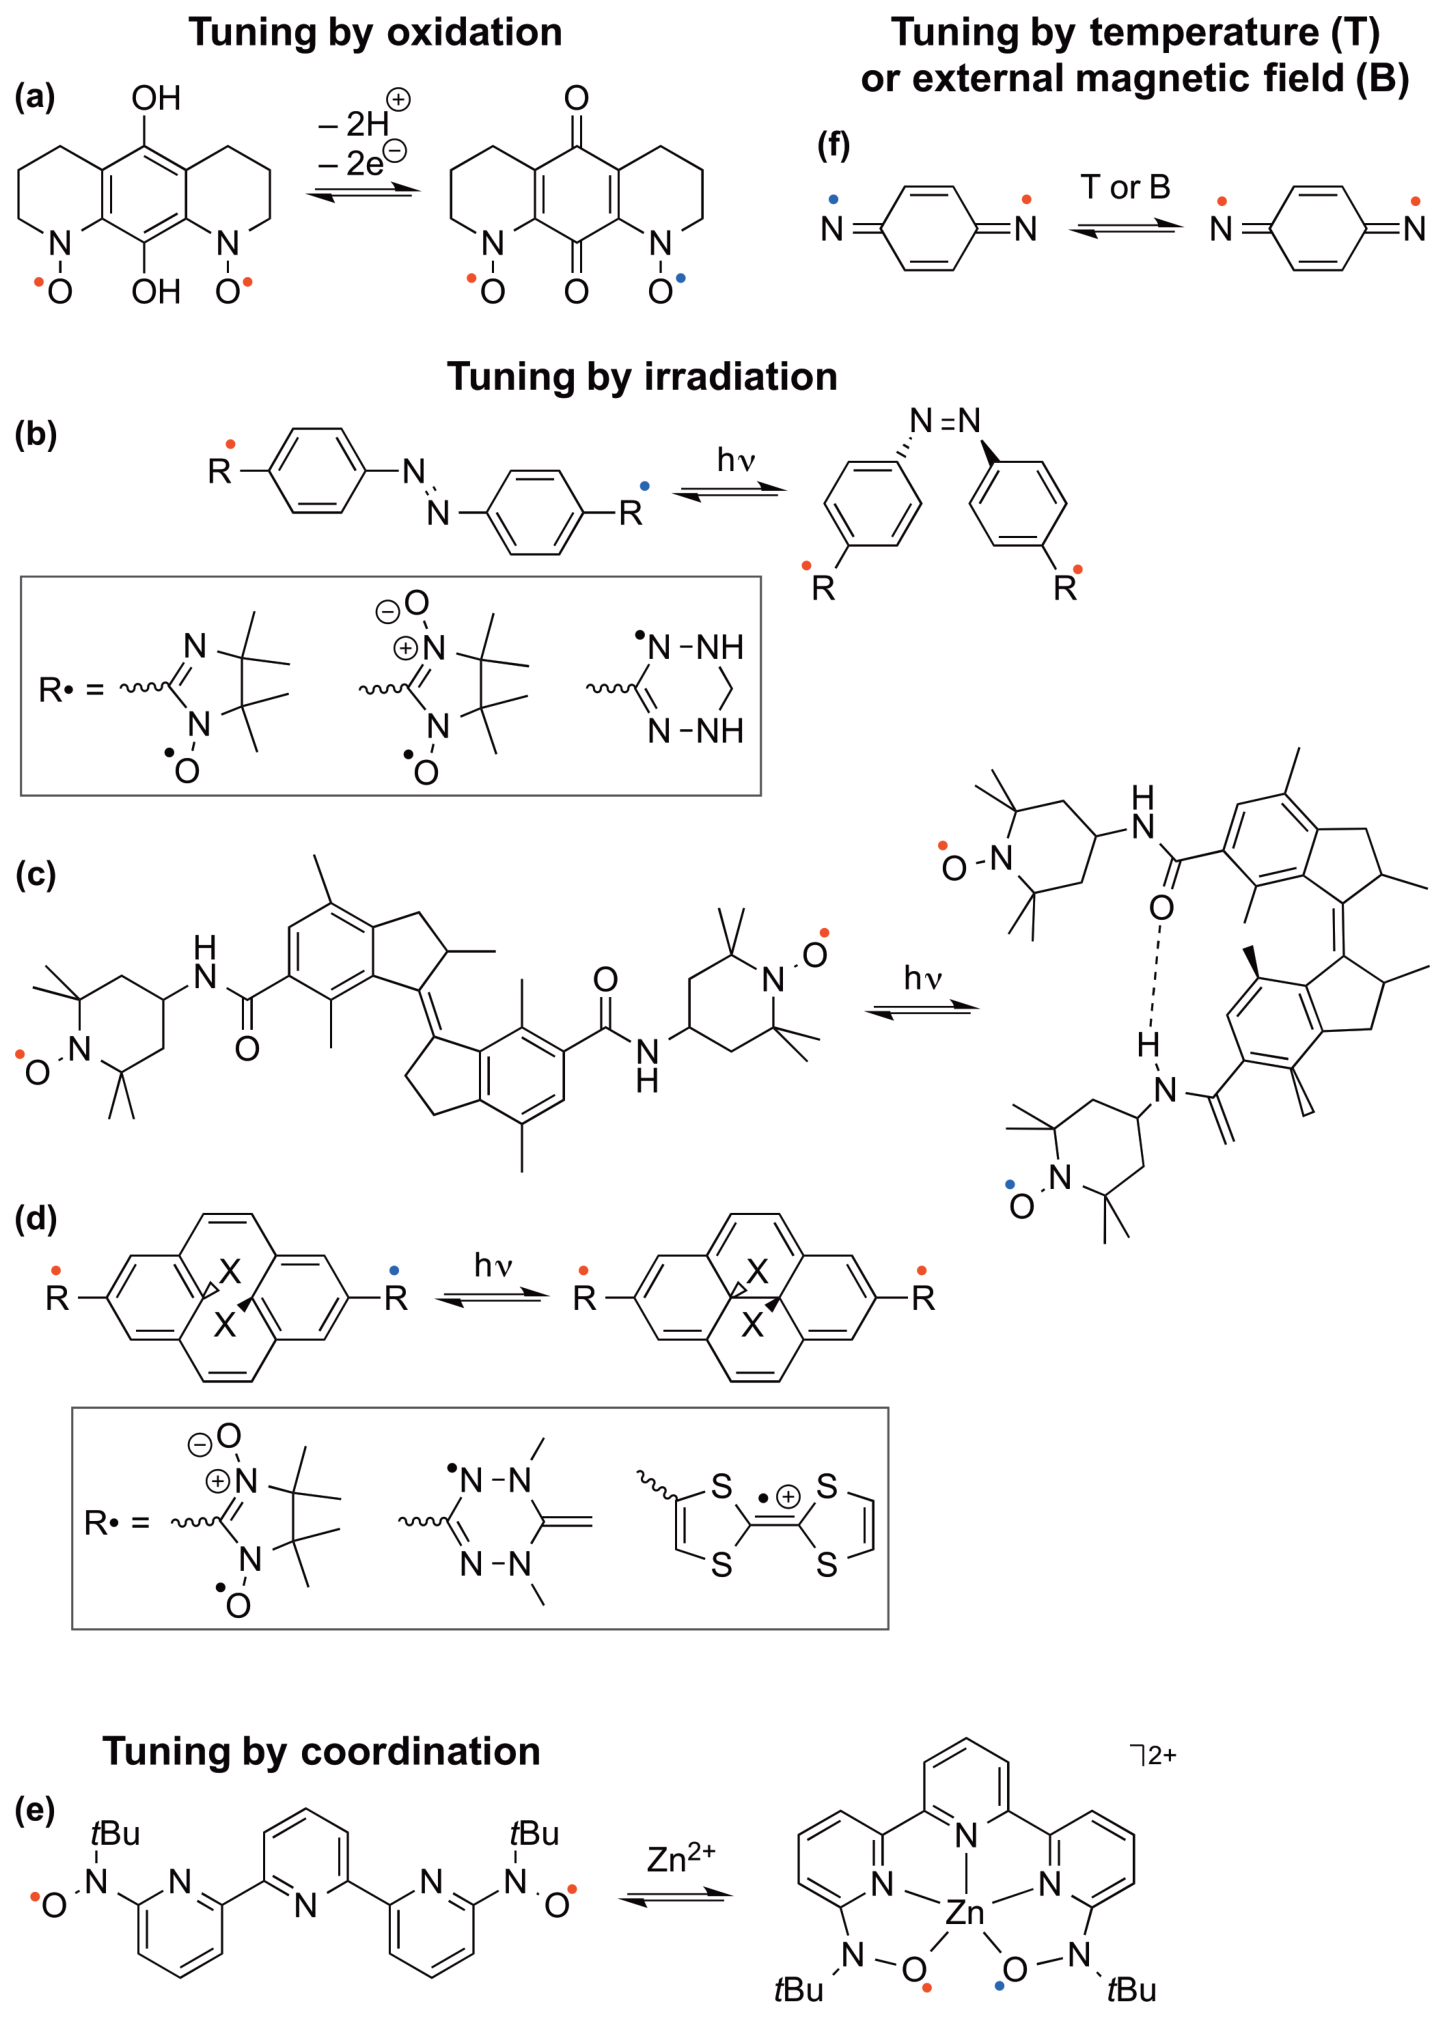
\includegraphics[height=0.74\textheight]{fig07_spin_crossover_external_stimuli.png}
    \column{0.55\textwidth}
    \footnotesize
    \begin{itemize}
      \item<1-> \cgold{(a) oxidation}: quinone coupler switches two nitroxides between ferro- and antiferromagnetic coupling
      \item<2-> \cgold{(b) light}: \emph{cis}-azobenzene loses planarity, triplet $\to$ singlet (computed)
      \item<3-> \cgold{(c) light}: \emph{trans}$\to$\emph{cis} alkene brings two TEMPO units close, H-bonded, antiferromagnetic
      \item<4-> \cgold{(d) light}: photo-induced bond formation changes the orbital topology
      \item<5-> \cgold{(e) Zn$^{2+}$}: O--Zn--O superexchange and O$\cdots$O through-space exchange favour antiferromagnetic coupling
      \item<6-> \cgold{(f) $T$ or $B$}: 1,4-phenylenedinitrene, open-shell singlet $\to$ triplet
    \end{itemize}
  \end{columns}
\end{frame}

\begin{frame}{A wording slip in (e)?}
  \begin{paperclaim}
    ``Coordination to Zn$^{2+}$ brings about O--Zn--O superexchange and O$\cdots$O through-space exchange, which favor
    antiferromagnetic coupling and override the preference for the triplet ground state, predicted on the basis of
    \emph{disjoint} NBMOs in parent dinitroxide ligand'' (p.\ 445)
  \end{paperclaim}
  \begin{columns}[T]
    \column{0.48\textwidth}
    \onslide<2->{
    \begin{plainpanel}
      review, p.\ 443: \cgold{disjoint} NBMOs make the singlet \emph{competitive};
      a \cgold{triplet} preference needs \cgold{nondisjoint} NBMOs ($K>0$)
    \end{plainpanel}}
    \column{0.48\textwidth}
    \onslide<3->{
    \begin{plainpanel}
      so ``disjoint'' here is probably meant as ``nondisjoint'', or the triplet preference has another origin
    \end{plainpanel}}
  \end{columns}
  \vskip0.1cm
  \onslide<4->{\centering\warnpill\ \small inconsistent wording; \cmuted{original (ref.\ 52) not checked}\par}
\end{frame}

\begin{frame}{Panel (f), quantitatively: temperature}
  \begin{assume}
    open-shell singlet ground state, triplet $\Delta$ above it; Boltzmann statistics; degeneracies 1 and 3
  \end{assume}
  \begin{columns}[c]
    \column{0.5\textwidth}
    {\large
    \begin{align*}
      Z&=1+3e^{-\Delta/k_BT}\\
      \uncover<2->{p_T}&\uncover<2->{=\frac{3e^{-\Delta/k_BT}}{1+3e^{-\Delta/k_BT}}}\\
      \uncover<3->{p_T(T\to\infty)}&\uncover<3->{\to\tfrac34}
    \end{align*}}
    \onslide<4->{\small ``increased temperature \dots\ promotes electrons to populate the triplet state'' \okpill}
    \column{0.46\textwidth}
    \onslide<2->{
    \begin{tikzpicture}
      \begin{axis}[noirplot,width=6.4cm,height=4.8cm,xmin=0,xmax=4,ymin=0,ymax=0.8,
          xlabel={$k_BT/\Delta$},ylabel={$p_T$},ymajorgrids]
        \addplot[noirrose,very thick,domain=0.02:4,samples=100] {3*exp(-1/x)/(1+3*exp(-1/x))};
        \draw[noirmuted,dashed] (axis cs:0,0.75) -- (axis cs:4,0.75);
      \end{axis}
    \end{tikzpicture}}
  \end{columns}
\end{frame}

\begin{frame}{Panel (f), quantitatively: magnetic field}
  \begin{columns}[c]
    \column{0.5\textwidth}
    \begin{assume}
      Zeeman term $g\mu_BBM_S$; singlet unaffected; $g\approx2$
    \end{assume}
    {\large
    \begin{align*}
      E_T(M_S)&=\Delta+g\mu_BB\,M_S,\quad M_S=0,\pm1\\
      \uncover<2->{E_T(-1)=E_S}&\uncover<2->{\ \Leftrightarrow\ B^*=\frac{\Delta}{g\mu_B}}
    \end{align*}}
    \onslide<3->{\small ``external magnetic field that splits the triplet into microstates, one of which approaches the energy of the
      ground-state singlet'' \okpill}
    \column{0.46\textwidth}
    \begin{tikzpicture}
      \begin{axis}[noirplot,width=6.4cm,height=5.2cm,xmin=0,xmax=1.5,ymin=-0.6,ymax=2.6,
          xlabel={$g\mu_BB/\Delta$},ylabel={$E/\Delta$},ymajorgrids]
        \addplot[noirblue,very thick,domain=0:1.5] {0};
        \only<1->{\addplot[noirrose,very thick,domain=0:1.5] {1+x};
                  \addplot[noirrose,very thick,domain=0:1.5] {1};
                  \addplot[noirrose,very thick,domain=0:1.5] {1-x};}
        \only<2->{\draw[noirgold,dashed] (axis cs:1,-0.6) -- (axis cs:1,2.6);}
        \node[font=\scriptsize,text=noirblue,anchor=south west] at (axis cs:0.02,0.02) {$S$};
        \node[font=\scriptsize,text=noirrose,anchor=south west] at (axis cs:0.02,1.05) {$T$};
      \end{axis}
    \end{tikzpicture}
  \end{columns}
\end{frame}

\begin{frame}{Closed shell or diradical? (Figures 8 and 9)}
  \begin{columns}[c]
    \column{0.4\textwidth}
    \centering
    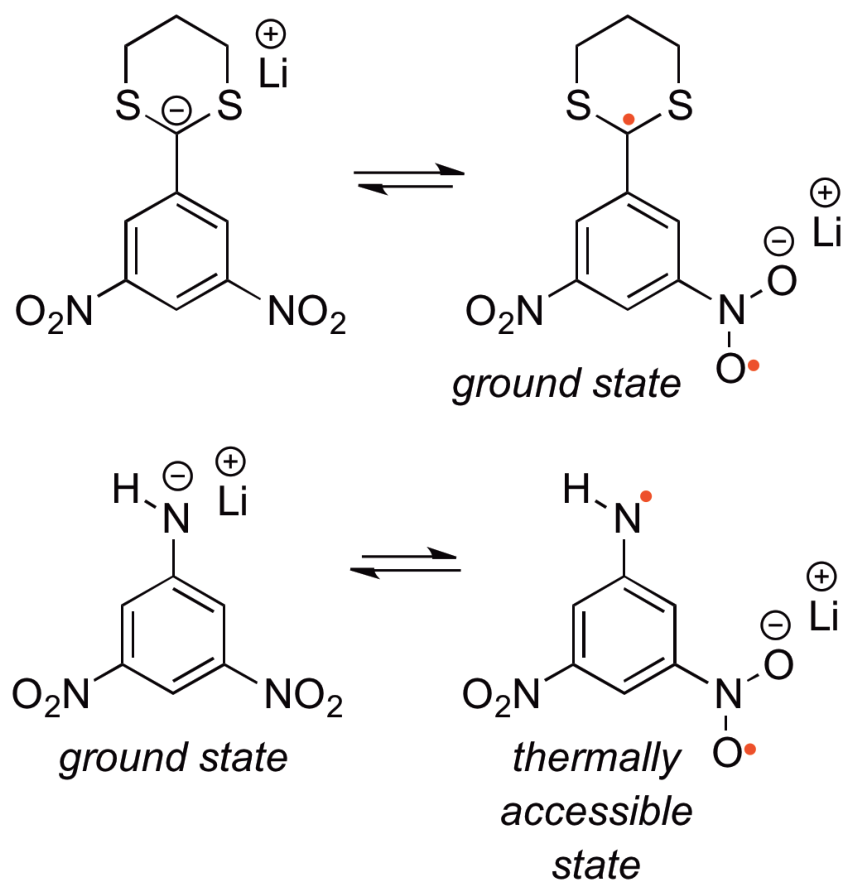
\includegraphics[width=0.9\linewidth]{fig08_borderline_triplet_closed_shell.png}
    \column{0.57\textwidth}
    \small
    \begin{itemize}
      \item \cgold{Fig.\ 8}: 1,3-dinitrophenyls with anionic substituents transfer an electron intramolecularly to give
        anionic diradicals; triplet is the ground state or only negligibly above the closed shell; cation binding to the
        nitro group stabilises the diradical
      \item<2-> \cgold{Fig.\ 9}: protonation (and oxidation) creates diradicals: donor--acceptor electron transfer after
        double protonation, a sapphyrin-derived singlet biradicaloid, a dipyrylium diradical salt, high-spin building blocks
        for polaronic ferromagnets
      \item<3-> \cgold{singlet fission}: one excited singlet shares its excitation with a neighbour; both end in a low triplet
    \end{itemize}
  \end{columns}
\end{frame}

\begin{frame}{Protonation-induced magnetisation (Figure 9)}
  \centering
  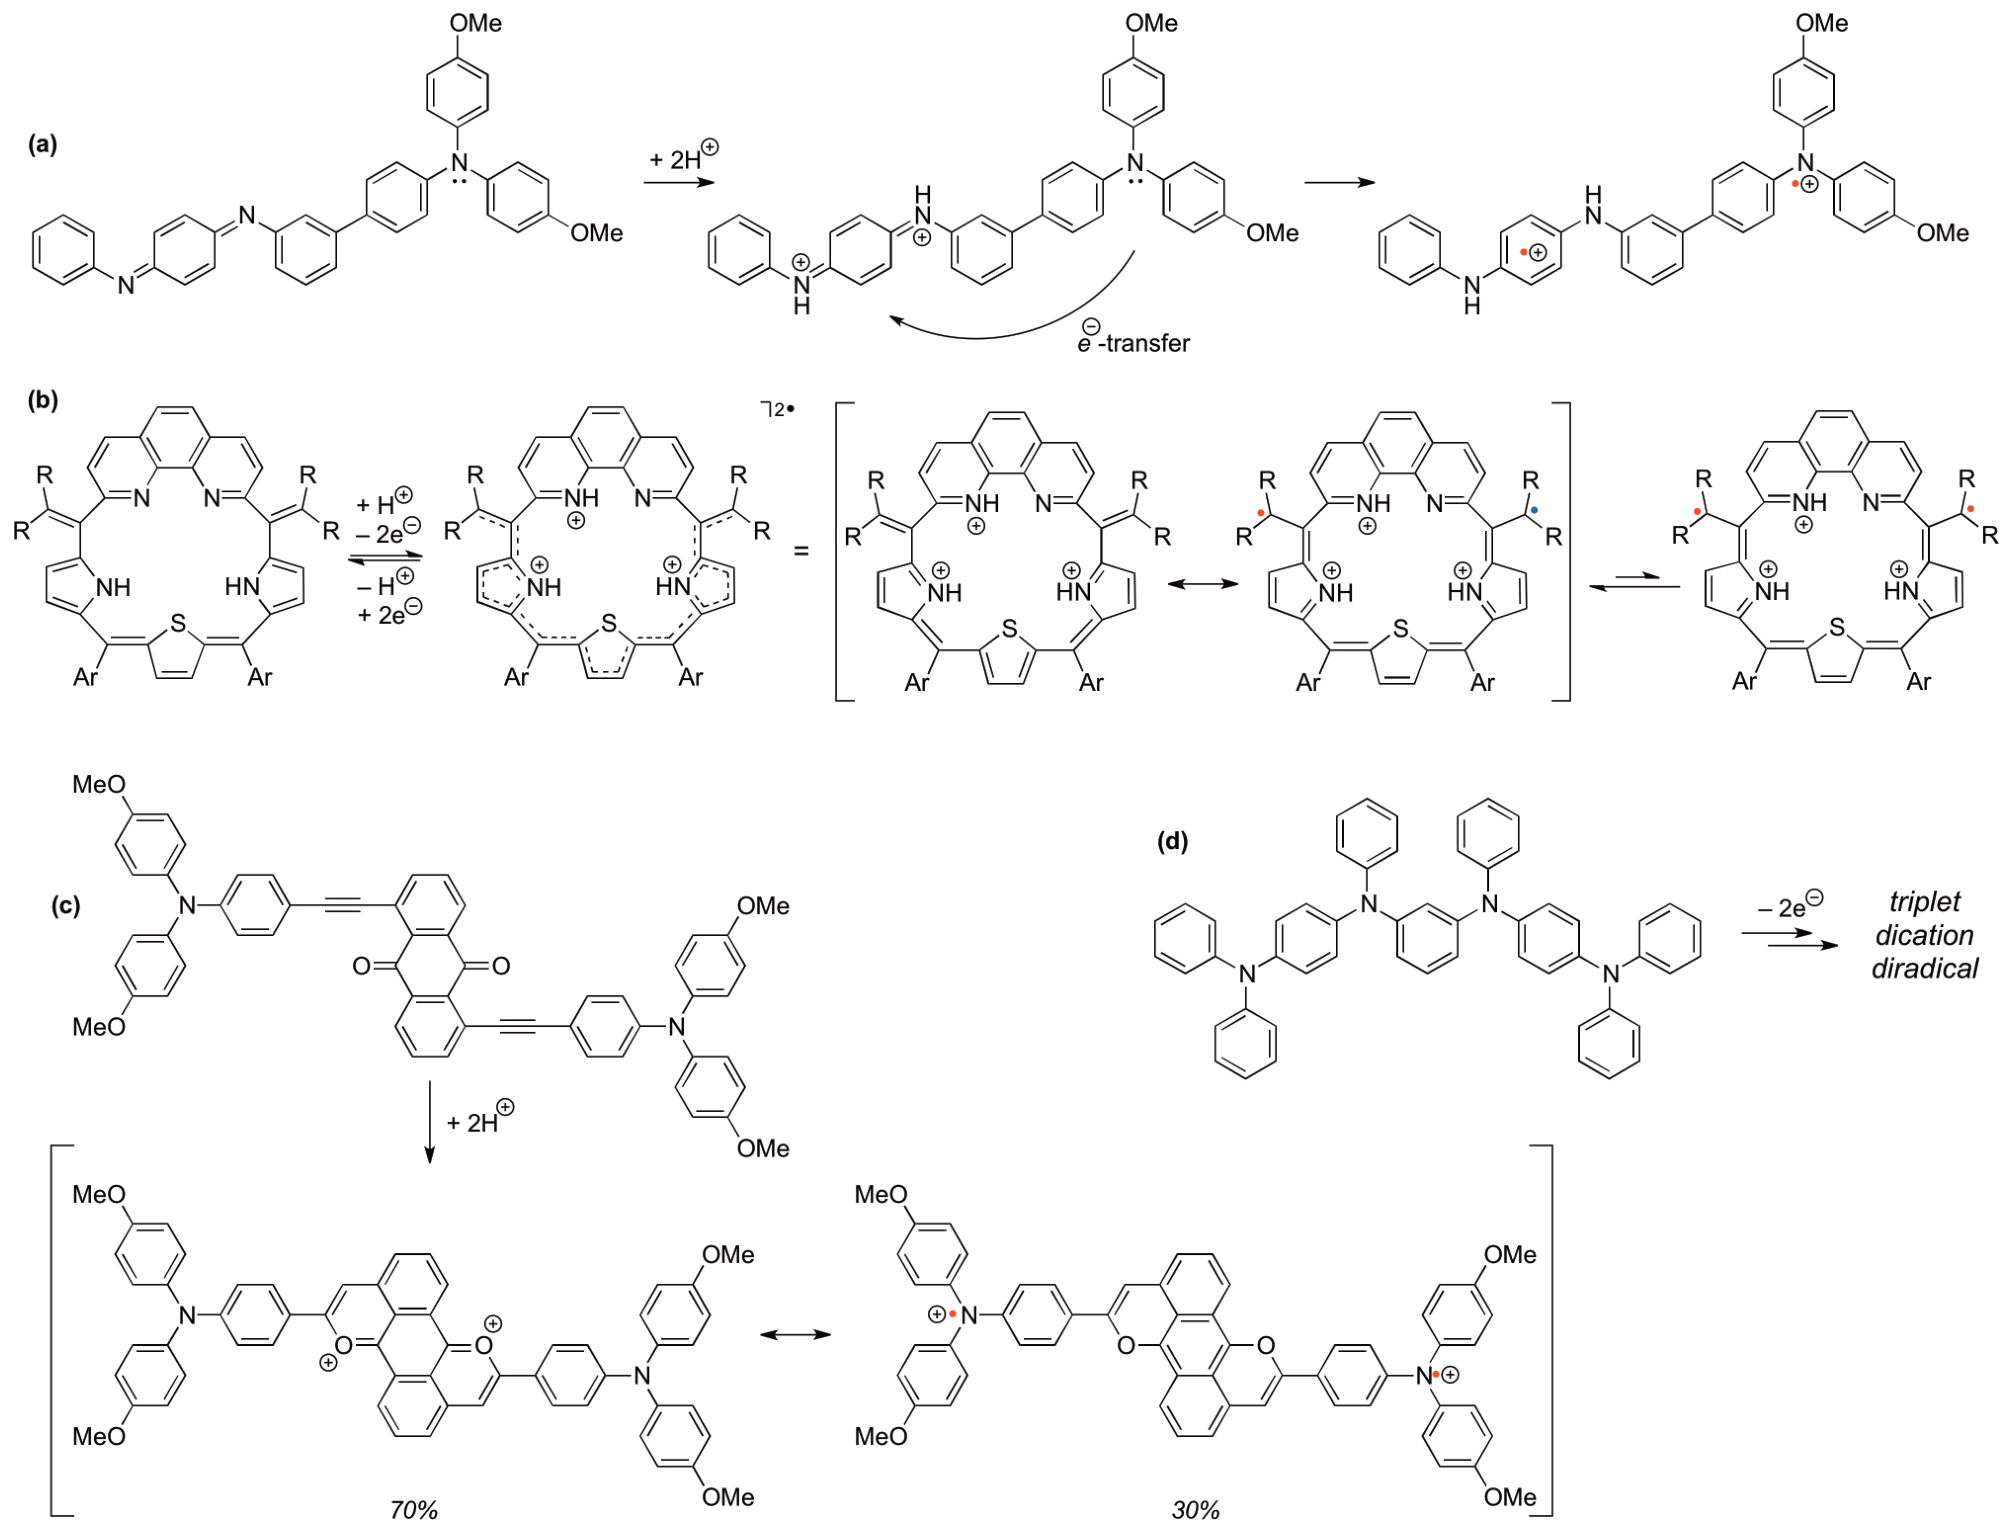
\includegraphics[height=0.64\textheight]{fig09_protonation_induced_magnetization.png}
  \vskip0.1cm
  {\small\cmuted{descriptive part of the review: no mathematics to derive, only claims about specific molecules (not re-checked)}}
\end{frame}
